\section{Operating systems}

\begin{description}
		\item[Node-centric operating systems] Simplified versions of normal
				operating systems, providing abstraction of node to
				programmers. Example: MANTIS, RIOT.
		\item[Node-level progrmaming tools] Platform providing components to
				programmer. Example: TinyOS, Contiki.
\end{description}

\subsection{Concurrency}

\begin{description}
		\item[True vs pseudo] Multi-process (requries multiple processors) vs
				sequential
		\item[Event-driven] Kernel invokes event handlers when
				event occurs. One event runs at a time. Event
				handler runs to completion.
				\begin{itemize}
						\item Cheap pseudo-concurrency, complements networking protocols, inexpensive
						\item Program must be chopped into subprograms, high learning curve
				\end{itemize}
		\item[Multi-threading] Threads are waiting for events.
				Kernel unblocks threads when event occurs.
				Threads run until next blocking statement. Each
				thread requires stack, but long operations
				possible.
				\begin{itemize}
						\item Programmer in control. Real-time performance.
								Better simulation of true concurrency.
						\item High memory footprint. Complex shared memory.
								Expensive context switches.
				\end{itemize}
		\item[Mix: Threads on top of event-driven kernel] Kernel is
				event-based, multi-threading as library, used by tasks where
				required.
\end{description}

\subsection{TinyOS}

\begin{itemize}
		\item Simplifications: No FS, static memory allocation, thread support by application level library, minimal network abstractions
		\item Each application built into the operating system
		\item Concurrency left to programmer, event model
		\item Applications written in nesC, static language (no dynamic memory allocations!), support for even-tbased TinyOS design
		\item Events: Interrupts by clock, radio, ..., execute event handlers which run to completion
		\item Tasks: Created by component, posted to task scheduler. Run to completion, a form of deferred computation.
		\item Separation of method call initiation and return of call, compare async methods
		\item Commands flow to lower components, events back to higher ones
\end{itemize}

\subsection{ContikiOS}

\begin{itemize}
		\item Event-driven kernel with preemptive multitasking
		\item Core OS as binary image, programs loaded by loader
		\item Kernel dispatches events to processes, which define event handlers and optional polling handlers to poll hardware state
		\item Process state stored in its own memory. Processes share address space, no memory protection.
		\item Event scheduler handles async and sync events. Async are
				dispatched at some point, synchronous execute event handler
				immediately, then return.
		\item Event handlers run to completion
		\item $\mu$-IP, small TCP/IP stack with support for IPv4/6. Largely RFC-compliant.
\end{itemize}

\subsubsection{Protothreads}

\begin{itemize}
		\item Stackless
		\item Local variables not preserved across blocking statements
		\item But no need to run to completion, as only have to run to next blocking statement
\end{itemize}

\subsection{MANTIS OS}

\begin{itemize}
		\item Layered multi-threaded OS. Nearly a full OS.
		\item Global variables allocated at compile time, rest managed as heap. Stack for each thread frmo heap.
		\item Fixed size thread table.
		\item HW interrupts sent to drivers. No SW interrupts. Timer interrupts handled by kernel.
		\item Different options for network stack.
		\item Power management via sleep. When all threads asleep, OS shuts down microcontroller.
		\item Dynamic reprogramming possible. (eg OTA)
\end{itemize}

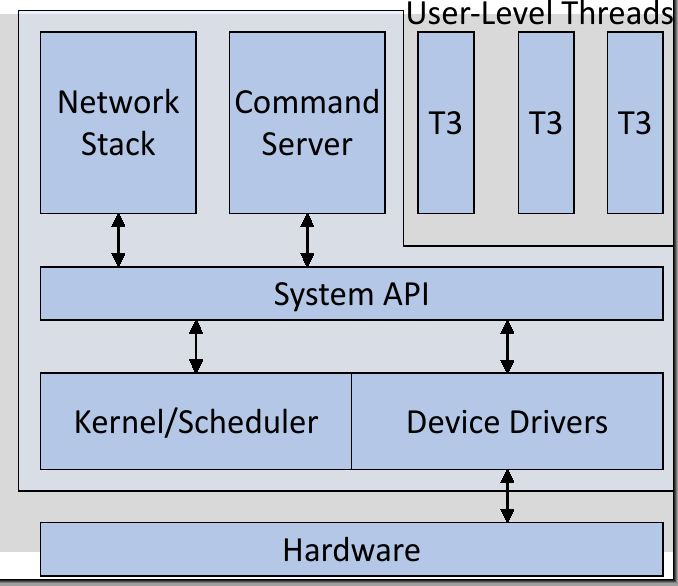
\includegraphics[width=0.5\textwidth]{03_mantis}

\subsection{RIOT}

\begin{itemize}
		\item Microkernel with multithreading
		\item Static memory allocation
		\item TCP/IP stack
		\item Scheduler switches to idle (sleep) thread when nothing to do,
				wakes up on interrupts (external or kernel-generated)
\end{itemize}

\subsection{OS power management}

\subsubsection{Low-Energy Earlierst Deadline First Scheduling (LEDF)}

CPU-centric.

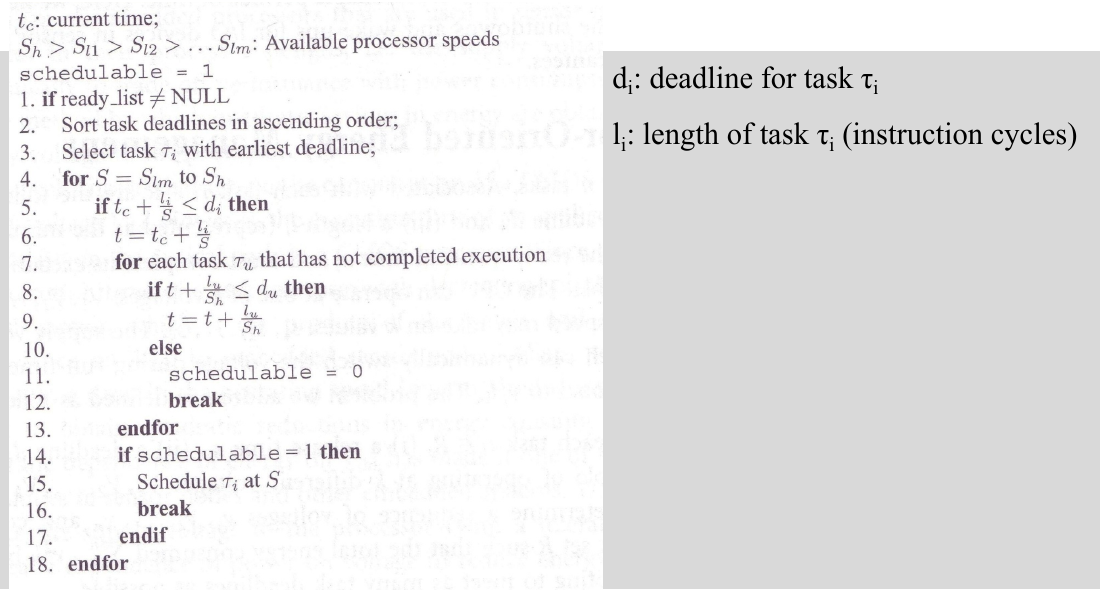
\includegraphics[width=\textwidth]{03_ledf}

\subsubsection{Low-Energy Device Scheduling (LEDES)}

I/O-centric.

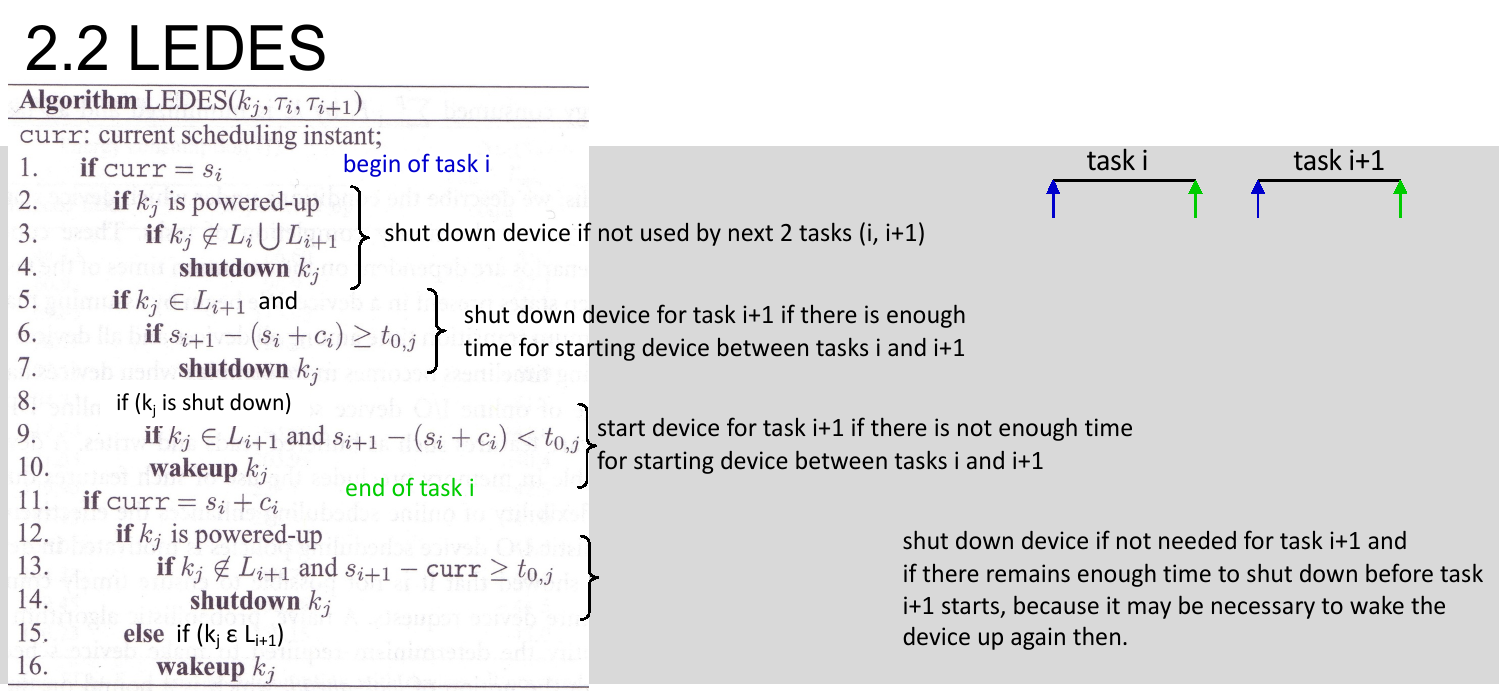
\includegraphics[width=\textwidth]{03_ledes}
